\chapter{The socio-technical system of \textit{DrupalCons}}
\chaptermark{``Mostly-offline" contributions: \textit{DrupalCons}}
\label{mostly-offline-cons:chapter}

This chapter concludes the study of socio-technical systems of contribution with the exploration of the system of \textit{DrupalCons}. As it was introduced in section \ref{sec:growth-community}, \textit{DrupalCons} are major international Drupal events whose latest editions have been attended by thousands of Drupalistas. \textit{DrupalCons} include a vast and varied set of activities: peer-reviewed presentations, keynotes by Dries and other famous speakers  from other FLOSS or technological communities or organisations\footnote{For example Fabien Potencier (Symfony), Cory Doctorow (Electronic Frontier Foundation), Mitchell Baker (Mozilla Foundation), Rasmus Lerdorf (PHP) or Senator Kate Lundy (Australian Ministry for Industry and Innovation).}, ``BoFs" (Birds of a Feather), community summits, code sprints, or social events among others.

Following a structure similar to that seen in previous chapters, section \ref{subsec:dcons-emergence} initially provides an overview of the emergence of this socio-technical system and its main organisational aspects during this initial stage. Subsequently, section \ref{subsec:dcons-growth} explores a transitional period in which ``\textit{DrupalCons} used to be like \textit{DrupalCamps}". The growth and massive changes experienced by the events over this period produced the rise of a new type of event, ``modern \textit{DrupalCons}", whose changes were intertwined with a shift in the legitimacy to hold these events placed in the hands of the most formal and centralised institution in the community: the Drupal Association.

In order to illustrate how the general dynamics of formalisation and decentralisation operate in this socio-technical system of ``modern \textit{DrupalCons}", an analogous structure as that formerly employed for the exploration of \textit{DrupalCamps} will follow in section \ref{subsec:dec-form-modern-dcons} through a case study.  Firstly, the general organisational characteristics and changes experienced over time in this socio-technical system are explored within the context of those experienced by the Drupal Association. Secondly, throughout the same case study, the selection of presentations in current \textit{DrupalCons} is explored, in order to offer an in-depth exploration of how the aforementioned general dynamics of formalisation and decentralisation operate in the day-to-day of this socio-technical system of contribution, while also allowing the comparison of these self-organisational processes with those previously explored for all other socio-technical systems of contribution.


\section{Emergence of \textit{DrupalCons}}
\label{subsec:dcons-emergence}

\textit{DrupalCons} originated from the first international meeting of Drupalistas in Belgium in 2005 --- see section \ref{subsec:offline-side}. This first event is considered by some Drupalistas as the first \textit{DrupalCon}, as illustrated by the following excerpt from I\textunderscript{4}, one of the attendees:

\begin{quotation}
``[...] the first DrupalCon we had was actually in Antwerp, just because Dries was studying there, [...]. So there wasn't presentations. It was just kind of F2F discussions, people getting together to do some coding together, and kind of create some prototypes and getting ideas together and whatever. And kind of forward-planning. Doing that kind of planning F2F it was way, way better than doing it online."

\begin{flushright}\footnotesize{Developer and project manager, organiser of local events and \textit{DrupalCamps}, M, 11 years.}\end{flushright}
\end{quotation}

The previous excerpt also illustrates another relevant aspect: the high degree of informality of these events at this early stage. The dynamics of these initial events resemble those presented in section \ref{subsec:local-events} for current local events, such as Drupal Code sprints or Drupal Show and Tells. They were largely informal, participant-driven and fluid, depicting similar characteristics to those of hackathons and unconferences \parencite[9-10]{greenhill2008unconference}. This informality was also reflected in the organisational processes of these events. The following excerpt, in figure \ref{dcon2006}, depicts the thread\footnote{In these first events there were not even specific websites created for them. The main artefact for collaboration were pages at Drupal.org. For example, for this specific event, an announcement at \url{https://www.drupal.org/node/74812} and a page in a Drupal group at \url{https://groups.drupal.org/drupalcon-brussels-2006}.} opened by Dries asking for suggestions to organise the \textit{DrupalCon} in Europe the year after, illustrating informality in the organisation and the growth in attendance:

\begin{figure}[H]
  \centering
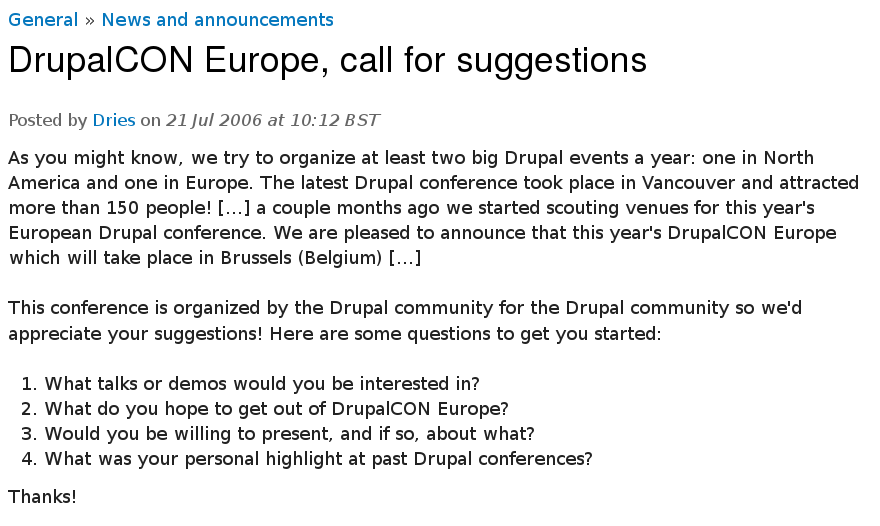
\includegraphics[width=\textwidth]{img/quotes_replacement/dcon_2006_dries.png}
\caption[Excerpt from ``\textit{DrupalCON} Europe, call for suggestions"]{Excerpt from ``\textit{DrupalCON} Europe, call for suggestions". Retrieved \nth{8} May 2017, from \url{https://www.drupal.org/node/74812}.}
\label{dcon2006}
\end{figure}

Some of the comments made in this thread by other Drupalistas also illustrate the high degree of informality in decision-making at the time. There were no formal rules or structures for decision-making, and the process was carried out following the purest forms of ``do-ocracy". Consensus was reached via online discussion, in what was still a small and informal network of people. Members could trust each other and carry out decision-making and quality assurance without requiring more formal structures. These dynamics also resembled the primal dynamics seen in the case of \textit{core} projects in their earliest stages. For example, the following two comments on the discussion of the announcement depict how presentations were informally proposed, and how the selection of presentations was encouraged by Dries to be carried out in collaborative, although rudimentary, ways:

\begin{figure}[H]
  \centering
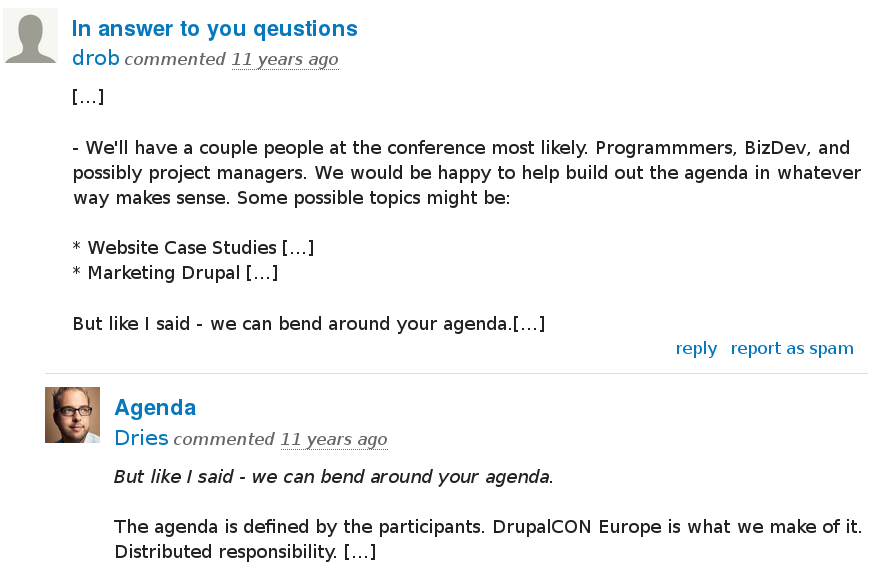
\includegraphics[width=\textwidth]{img/quotes_replacement/dcon_brussels_2016_comments.png}
\caption[Excerpt from comments (I) on ``\textit{DrupalCON} Europe, call for suggestions"]{Excerpt from comments (I) on ``\textit{DrupalCON} Europe, call for suggestions". Retrieved \nth{8} May 2017, from \url{https://www.drupal.org/node/74812}.}
\label{dcon2006_comments01}
\end{figure}

Over subsequent comments in the same announcement, it can also be shown how these incipient quality assurance mechanisms drew on the reputation of a still informal, small group of Drupalistas. Mechanisms at this stage were lacking transparency, objectivity and standarisation. In this environment, those well-known contributors were easily recognisable and, even when preferential treatment was given to some well-known and trusted members, no conflicts or tensions arose. Figure \ref{dcon2006_comments02} depicts, for example, how two slots for presentations by \textsl{merlinofchaos}\footnote{\textsl{Merlinofchaos} (\url{https://www.drupal.org/u/merlinofchaos}) is a historic member of the Drupal community and major contributor. Among many other contributions, he is the main developer behind one of the most important \textit{contributed} projects in the history of Drupal: \textit{views}. Due to its relevance, this module was incorporated as part of Drupal 8 core through a Core Initiative.} were directly appointed by Dries. Furthermore, as depicted by the comment below, other users wanted more presentation slots for him:


\begin{figure}[H]
  \centering
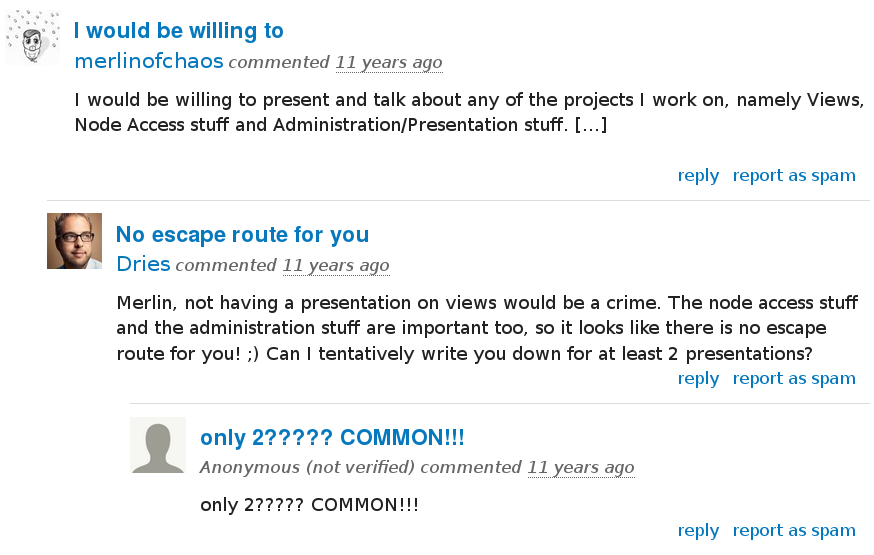
\includegraphics[width=\textwidth]{img/quotes_replacement/dcon_brussels_2016_comments02.png}
\caption[Excerpt from comments (II) on ``\textit{DrupalCON} Europe, call for suggestions"]{Excerpt from comments (II) on ``\textit{DrupalCON} Europe, call for suggestions". Retrieved \nth{8} May 2017, from \url{https://www.drupal.org/node/74812}.}
\label{dcon2006_comments02}
\end{figure}

Overall, these excerpts demonstrate the high degree of informality of a socio-technical system in an incipient state: operating on the most ``do-ocratic" basis and whose dynamics resemble those of today's most informal socio-technical system of events. The number of participants was low, the decision-making was regulated by informal social rules, in which the opinions of those with a highly regarded reputation in the community (e.g. Dries or \textsl{merlinofchaos}) were more prominent.

\section{Growth of \textit{DrupalCons}: ``\textit{DrupalCons} used to be like \textit{DrupalCamps}"}
\label{subsec:dcons-growth}

As the number of Drupalistas involved in the community continued to grow,  the organisational processes which surrounded these events became more formalised. After several editions, the organisational processes which surround \textit{DrupalCons} evolved in an analogous manner comparable to those of recent \textit{DrupalCamps}. For instance, more formalised and explicit rules for decision-making and a clearer division of labour were defined. These changes were reflected in the artefacts employed for collaboration. The website created specifically for \textit{DrupalCon} Boston in 2008 illustrates, for example, this clearer definition of rules with regard to the quality assurance processes for the selection of presentations for one of the tracks:

\begin{figure}[H]
  \centering
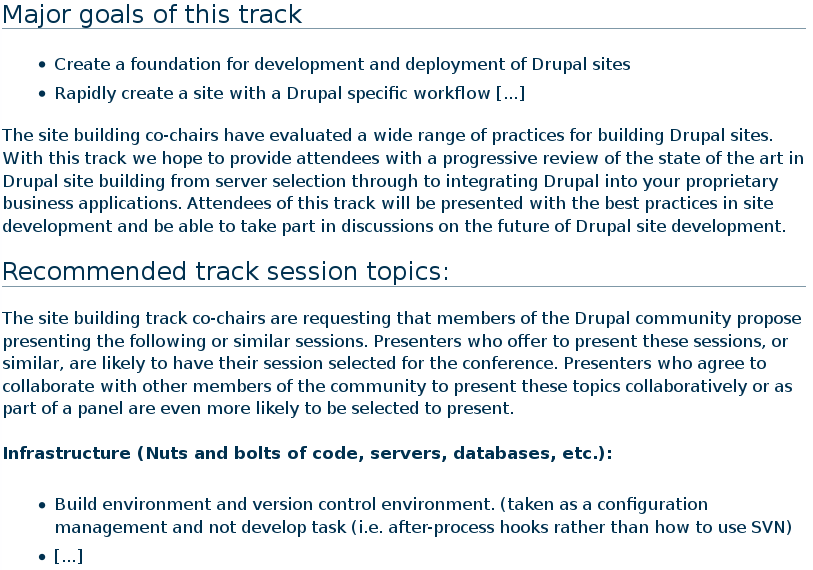
\includegraphics[width=\textwidth]{img/quotes_replacement/dcon_boston_01.png}
\caption[Excerpt (I) from ``Site building track descriptions" at \textit{DrupalCon} Boston 2008]{Excerpt (I) from ``Site building track descriptions" at \textit{DrupalCon} Boston 2008,  depicting clearer rules. Retrieved \nth{12} May 2016, from \url{http://boston2008.drupalcon.org/site-building-track-descriptions.html}.}
\label{dcon_boston01}
\end{figure}

Similarly, with regards to the division of labour, this increase in the degree of formalisation can be seen in the figure of co-chairs, who acted as quality assurance gatekeepers for each track. The following excerpt provides evidence of this, using the same track (site building) as an example:

\begin{figure}[H]
  \centering
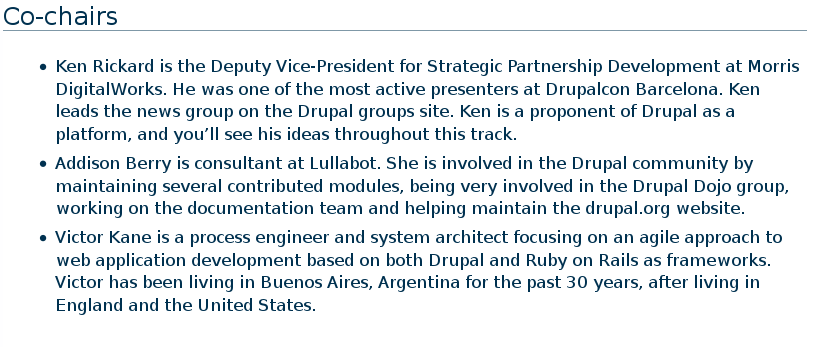
\includegraphics[width=\textwidth]{img/quotes_replacement/dcon_boston_02.png}
\caption[Excerpt (II) from ``Site building track descriptions" at \textit{DrupalCon} Boston 2008]{Excerpt (II) from ``Site building track descriptions" at \textit{DrupalCon} Boston 2008,  depicting clearer division of labour. Retrieved \nth{12} May 2016, from \url{http://boston2008.drupalcon.org/site-building-track-descriptions.html}.}
\label{dcon_boston02}
\end{figure}

These changes in the self-organisational processes for the selection of presentations for \textit{DrupalCons} at the time should be understood as part of the general dynamics of formalisation and decentralisation that shaped them, leading to the emergence of a socio-technical system of contribution whose organisational characteristics at the time more greatly resembled those of current \textit{DrupalCamps} presented in sections \ref{subsec:org-camps} and \ref{subsec:dcamps-emergence-local-institutions}. For example, when comparing the processes of quality assurance for the selection of presentations with the previous stage, the definition of peer-reviewing mechanisms and explicit collective-choice arrangements in the form of rules for decision-making appeared. This presents a higher degree of formalisation than in the first editions of \textit{DrupalCons} presented in section \ref{subsec:dcons-emergence}. Similarly, this entailed changes in the division of labour, with more specific roles, which also required stronger levels of legitimacy as the community grew, as in the case of current \textit{DrupalCamps}. This is illustrated, for instance, in the last excerpt of figure \ref{dcon_boston02} by the inclusion of credentials for the involvement and contributions of those who carried out the selection, in order to increase legitimacy. Nevertheless, as in the case of current \textit{DrupalCamps}, explicit collective-choice arrangements to select those who select were not yet formally defined at the time.

The changes experienced in the organisational processes of \textit{DrupalCons} at the time should also be understood in the context of the incipient foundation of the Drupal Association in 2007 --- see section \ref{subsec:foundation-da}. The emergence of an institution such as the Drupal Association can be understood as part of this general dynamic of formalisation, produced as a consequence of the need to scale up self-organisational processes and decision-making as the community grew; in a similar way to the vast emergence of local institutions for the case of \textit{DrupalCamps}, discussed in section \ref{subsec:dcamps-emergence-local-institutions}, but within a global scope. The jurisdiction for the organisation of \textit{DrupalCons} was, however, still more blurred at the time. \textit{DrupalCons} used to be organised by local communities, with the blessing of well-known members of the community before the existence of the Drupal Association, and with the blessing of the Drupal Association after its foundation. The following excerpt by I\textunderscript{10} summarises the organisational processes at the time:

\begin{quotation}
``[...] for the first several years, [...] someone would approach the Association, and say: `Hey, I wanna do a DrupalCon. Because I think it would be awesome to do it in my town'. And the Association would give their blessing. And pretty much it would list their name, and in return for, they [the Drupal Association] would get any profit from. Back then it was the local community doing its thing, and more or less was on its own."

\begin{flushright}\footnotesize{Drupal core developer and architect, M, 11 years.}\end{flushright}
\end{quotation}

However, as events continued to grow in attendance and organisational complexity, problems to scale up their organisation arose. As a response, a transition towards a clearer definition of boundaries started. This produced a shift in terms of jurisdiction, in which the Drupal Association centralised and accumulated more power. I\textunderscript{10}, member of the board of directors of the Drupal Association at the time, explained his view on the reasons why this shift was necessary:

\begin{quotation}
``[...] We were burning out local teams. It sometimes worked, sometimes didn't. [DrupalCon] Paris [2009] was kind of a disaster, because the local team didn't get their act together at all. [...] So after Paris, we made the decision to transition to the Association actually running these things. [...] Chicago [2011] I'd say was the first modern DrupalCon, where the Association run it. There was a local team, but the Association owned the process [...]"

\begin{flushright}\footnotesize{Drupal core developer and architect, M, 11 years.}\end{flushright}
\end{quotation}

At first glance, this could be understood as a clear counter-example of the general process of decentralisation due to the reduction in the autonomy of local communities with regard to the organisation of these events. However, a more detailed inspection of the characteristics and outcomes of these events from a macro perspective, indicates that this could be understood as a process of transition in which two different socio-technical systems of contribution activities emerged. In a similar way as in the case of the socio-technical systems of \textit{contributed} and \textit{core} projects in ``mostly-online" activities, the higher degree of coordination and consistency of \textit{DrupalCons} entailed the emergence of these new types of ``modern" \textit{DrupalCons}, whose role is different from earlier editions. At the same time, the previous space was replaced by that of the socio-technical system of \textit{DrupalCamps}, which represents overall a much more autonomous, organic and decentralised space.  The following excerpt by I\textunderscript{11} illustrates how \textit{DrupalCamps} ``filled in" this space, in the context of a conversation about the differences between the outcomes of these events with respect to the creation of a sense of community:

\begin{quotation}
``[...] in Paris [2009] we were 600 people. Now it's what? 3,000 or something. [...] The biggest change is, because of size, it's maybe a different atmosphere. [...] in Paris, you know, DrupalCon felt more like a DrupalCamp now. In terms of the closer community feel. And, obviously, on the large scale there are ... it feels less close community. [...] when you go to an event where you're seeing the same faces every, maybe half an hour to an hour, it's a very different feeling as humans, [compared] to go to something where there's 3,000 people. [...] DrupalCons have kind of lost something when they got bigger in terms of being a community event. But I think they gained something, because they got the Camps to fit into that."

\begin{flushright}\footnotesize{Project manager, organiser of local events and \textit{DrupalCamps}, and volunteers' coordinator at several DrupalCons, M, 9 years.}\end{flushright}
\end{quotation}

As in the emergence of local institutions presented in section \ref{subsec:dcamps-emergence-local-institutions}, a shift like this, although within a global scope in this case, was not free of tensions. A global CBPP institution, such as the Drupal Association, requires the highest degrees of transparency, accountability and openness to participate in order to create legitimacy. As it will be shown in section \ref{subsec:dec-form-modern-dcons}, the changes experienced over time indicate this trend. However, in its origin, the organisational processes were more closed and centralised. The following excerpt by I\textunderscript{5}  shows this contrast with respect to the degree of transparency of decision-making in current \textit{DrupalCons}:

\begin{quotation}
``[...] Nowadays [the organisation of DrupalCons] is more open. [...] In Paris [2009] and Copenhagen [2010] a lot of the work was still carried out by the local communities as volunteers. And, after that, the Drupal Association took control. And, I believe, for some years, and as a consequence of this change, the processes were much more closed."

\begin{flushright}\footnotesize{Drupal developer and ex-member of the Drupal Association Board of Directors, M, 9 years. Original reply in Spanish.}\end{flushright}
\end{quotation}

The tensions due to the concentration of power in the hands of a global institution, to the detriment of local communities, are still present to this day. For instance, this was reflected in the perceptions expressed by some Drupalistas during the participant observation, such as ``the Drupal Association being out of touch from their reality", or the common reference to the Drupal Association as ``they" --- even when they are members --- while to the community as ``we". Other examples of the reflection of these tensions are the common criticisms\footnote{Another example of this tension was the discussion about the need to create a Drupal European Foundation. The initiative seems to be abandoned at the time of writing (May 2016), and the main website disappeared. Nevertheless, the original Twitter (\url{https://twitter.com/eudrupal}) and Facebook group account are still online (\url{https://www.facebook.com/europeandrupalfoundation}).} of the Drupal Association raised by some European Drupalistas during the observation for being ``too American and not representative of the community". The excerpt, extracted from field notes taken during participant observation at \textit{DrupalCon} Amsterdam 2014, illustrate how these types of tensions are still present in the day-to-day of the community:

\begin{quotation}
``[...] Similar issues were raised by some Drupalistas later, and I thought of this as a clear point of tension. For example, while having a chat outside with some Drupalistas, \textit{Pepe} was complaining about the fact that local communities have almost no voice in the organisation of DrupalCons. Some of them were even making some sarcastic jokes about it, using references to films: `leave it to the guys in black suits', or `they are like Mr. Wolf in Reservoir Dogs, they will come and sort everything out'. Another guy said he saw the point in them having more power overall, since these events are too big now. However, \textit{Pepe} insisted in the fact that the local community should have more influence. [...]
It seems to me this issue was related with the wider one of the dynamics of power in the community. For example, it reminded me of the discussion I had before with \textit{Joe} (a former member of the committee), after attending the Drupal Association public committee meeting. From his point of view, the boarding committee is not very willing to have a bigger influence from the community. He explained: `they mentioned they are becoming more effective, but effective for what purposes and interests?' [...] His impression was that `they' are afraid of the community having more power."

\begin{flushright}\footnotesize{Full field notes during observation at \textit{DrupalCon} Amsterdam (\nth{1} October 2014).}\end{flushright}
\end{quotation}

These tensions, due to the higher degree of centralisation of this socio-technical system of contribution, were also prominently found with regard to decision-making because of a lack of legitimacy accorded to local communities to participate in them under this more centralised structure. For instance, the excerpt below, from full field notes during the observation at the same event, illustrate this tension, in which a previous local organiser advised those in whose city the event would be held the next year to assume their lack of power to take the most relevant decisions:

\begin{quotation}
``[...] After attending that presentation, I bumped into \textit{Joe Lee} in the corridor. He told me that he couldn't tell me why, but I should go to a room at 15.45. Pretty mysterious moment! [...] It turned out that a `secret' meeting was called by the Drupal Association with some Spanish members of the Drupal community present in Amsterdam, because the next DrupalCon Europe will be held in Barcelona. They wanted some of them to participate in the official announcement. [...] Some of the Spanish Drupalistas were making some proposals, and asking about how the organisational processes work. \textit{Jokum}, who helped organised DrupalCon 2010 locally, stated it very clearly: `I tell you from my own experience. The sooner you realise that the Drupal Association has the control over the overall organisation of the event, the less painful it will be for you, guys'. The local teams help to organise it, and for instance they take care of the social events. Nevertheless, the key actor is the Drupal Association. [...] "

\begin{flushright}\footnotesize{Full field notes during observation at \textit{DrupalCon} Amsterdam (\nth{1} October 2014).}\end{flushright}
\end{quotation}

Hence, as in the case of the organisational processes related to ``mostly-online" activities, these processes are to be thought of as under a process of constant tension. In any case, the Drupal Association managed to successfully establish a sufficient degree of legitimisation, at least up to this day, regarding the organisation of these events in the eyes of many Drupalistas. Even when this led to a loss of autonomy for local communities. The following excerpt by I\textunderscript{11} illustrates an example of these views, which were commonly expressed by the Drupalistas interviewed:

\begin{quotation}
``[...] I think probably in the decision-making the local communities have lost some powers. But I don't think that's a bad thing. I think that the quality of the DrupalCons has improved based on that. Based on how big they are getting. [...]  there's a lot of thought processes, there's a lot of different decisions that are being made by the Association which I still think they are community-driven, but just in a sort of bigger way, if you see what I mean. Like a top-down way, rather than, you know, ... a local community running a DrupalCon just doesn't make any sense."

\begin{flushright}\footnotesize{Project manager, organiser of local events and \textit{DrupalCamps}, and volunteers' coordinator at several \textit{DrupalCons}, M, 9 years.}\end{flushright}
\end{quotation}

The emergence of this new socio-technical system of contribution of ``modern \textit{DrupalCons}" raises then another question. Was this socio-technical system of ``modern \textit{DrupalCons}" also affected by the dynamics of formalisation and decentralisation over time? Following a similar structure to that employed for the case study exploring \textit{DrupalCamps} in section \ref{subsec:dcamps-emergence-local-institutions}, over the next section the self-organisational processes of the socio-technical system of contribution of ``modern \textit{DrupalCons}" will be explored.

\section{Case study: formalisation and decentralisation in the organisation of ``modern \textit{DrupalCons}"}
\label{subsec:dec-form-modern-dcons}

In this section, the focus is placed on the study of organisational processes of ``modern \textit{DrupalCons}". The evolution of most of the processes during this stage was tightly coupled with those of the Drupal Association. As it will be shown, this was encompassed within a tendency towards a professionalisation of some of the tasks. This trend of professionalisation affects the dynamics of CBPP communities, since the main logic which operates in cases of professionalisation is based on contractual obligations rather than on self-assignation\footnote{While a general analysis of the evolution of the organisational practices when these hybrid forms of paid and unpaid labour in the community operate is of great interest, it would be more accurately framed from the perspective of studies on non-profit institutions or communities of organisations (further details will be discussed in section \ref{sec:conc:future-work}). Thus, it was out of the scope of this study.}, hence, contrary to one of the delimitation criteria presented in section \ref{subsubsec:state-art:cbpp:commons:cbpp} for CBPP communities. Nevertheless, the analysis of the processes relevant for this study, such as policy-making or quality assurance in \textit{DrupalCons}, were not part of this trend towards professionalisation. Thus, this will allow the comparison of its dynamics with those presented for the previous ``mostly-offline" socio-technical systems of contribution.

\subsection{Formalisation and professionalisation of the Drupal Association and effects on \textit{DrupalCons}}
\label{subsec:formalis-dcons}

As it was presented in the previous section, the growth of \textit{DrupalCons} led to a clearer definition of boundaries, explicitly stating that the jurisdiction for their organisation is in the hands of the Drupal Association. The changes that the organisation of \textit{DrupalCons} experienced from that point in time should be contextualised under a general period of transition in the overall governance model of the Drupal Association. A long discussion about the necessity to make the Drupal Association more transparent and accountable to the community had already started almost from its foundation. The debate became the most prominent during \textit{DrupalCon} San Francisco (2010), and organisational changes began to be implemented over the next year. The following excerpt provides an overview of the most relevant moments from the perspective of the Drupal Association at the time:

\begin{figure}[H]
  \centering
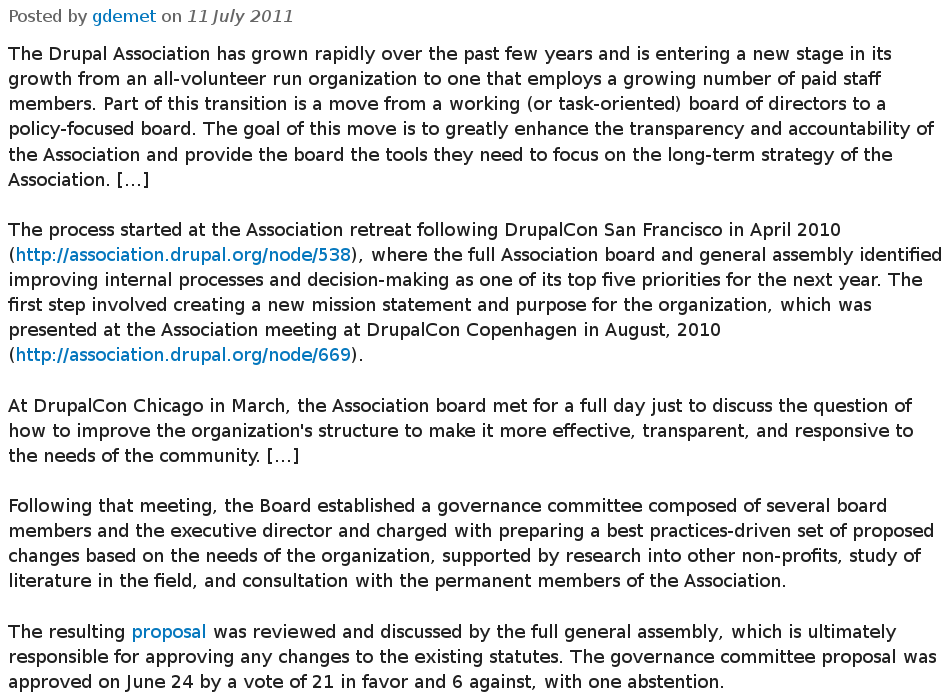
\includegraphics[width=\textwidth]{img/quotes_replacement/da_july2011.png}
\caption[Excerpt from the article ``Renewing the Organizational Structure of the Drupal Association"]{Excerpt from the article ``Renewing the Organizational Structure of the Drupal Association". Retrieved \nth{2} June 2016, from \url{https://assoc.drupal.org/node/1119}.}
\label{quote_renewing_da}
\end{figure}

The previous excerpt depicts two key aspects; firstly, the previously introduced trend of professionalisation for part of the tasks carried out by the Drupal Association. This shows a significant difference with respect to the way in which the previously presented socio-technical systems of contribution scaled up. While decision-making related to the creation of policies or quality assurance, as will be more exhaustively explored in this and in section \ref{subsec:dcons-day-to-day}, were not affected by this trend of professionalisation. The necessity to scale up organisational processes with regard to the maintenance of the main collaboration platform or part of the tasks related to \textit{DrupalCons} were also partially achieved by this means. This also entailed a discussion on what should or should not be considered as paid labour \parencite{drupal-volunteer-contractor:2016:Online}. After nearly three years of discussions, the line was drawn by providing a framework which left tasks which are more engaging --- those that ``scratch itches" using a FLOSS terminology --- for volunteers, while opening the door to contractors or staff for infrastructural and critical ones. The following excerpt depicts the character of the final set of guidelines from the perspective of the Drupal Association:

\begin{figure}[H]
  \centering
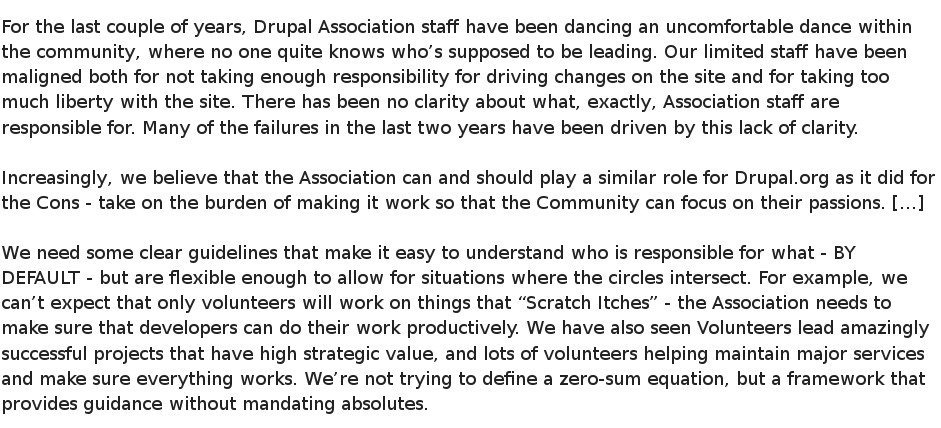
\includegraphics[width=\textwidth]{img/quotes_replacement/da_april2014.png}
\caption[Excerpt (I) from the article ``Defining Our Roles in the Drupal Community"]{Excerpt (I) from the article ``Defining Our Roles in the Drupal Community". Retrieved \nth{30} May 2016, from \url{https://assoc.drupal.org/content/defining-our-roles-drupal-community}.}
\label{quote_da_defining_roles_01}
\end{figure}

Overall, these organisational changes in the Drupal Association, despite their relation to the organisation of \textit{DrupalCons} or the management of Drupal.org,  should be understood as part of the general dynamic of formalisation in which clearer boundaries were defined, affecting the rules and the division of labour. Regarding decentralisation in decision-making over the tasks carried out by professional staff from the Drupal Association, the team was also significantly growing over time in order to scale up\footnote{The first professional was hired in 2010 \parencite{da-first-staff:2016:Online}, and the team grew to 25 people up to early May 2016. At the time of writing (May 2016), there was a recent announcement of the reduction to 17 employees, due to a lower growth in revenue than expected (14\%) \parencite{da-cuts:2016:Online}.}. However, since these activities are organised through contractual obligations, the evolution experienced by these organisational processes more greatly resembled the characteristics of a process of delegation commonly found in more traditional institutions. They represent a dispersal of authority, rather than the creation of autonomous and self-sufficient spaces. Hence, they will not be discussed under the general dynamic of decentralisation presented in this chapter. Instead, they were succinctly presented in order to contextualise the analysis of these dynamics of formalisation and decentralisation in other organisational processes around \textit{DrupalCons} under similar conditions, while also illustrating how they shaped the evolution of institutions, even for these hybrid cases in which part of the tasks are based on contractual obligations.

A second relevant aspect from the excerpt presented in figure \ref{quote_da_defining_roles_01} is the trend towards more open and accountable governance at the time. As in the case of the emergence of institutions for \textit{DrupalCamps} discussed in section \ref{subsec:dcamps-emergence-local-institutions}, in its origin the Drupal Association was perceived by many Drupalistas as opaque and lacking accountability, generating a series of tensions. For instance, some of these tensions were due to some Drupalistas feeling that the possibility to participate in the modification of collective-choice arrangements decreased, and strongly criticised the lack of transparency and accountability of the Drupal Association. These tensions should be understood within a context in which the legitimacy of these institutions for decision-making is under a process of constant scrutiny by the community. An example of this can be found in the discussion created around an article --- see figure \ref{quote_da_dcon_la_announcement} ---  about the process of selection of the location for the first \textit{DrupalCon} Latin America (2015).

\begin{figure}[H]
  \centering
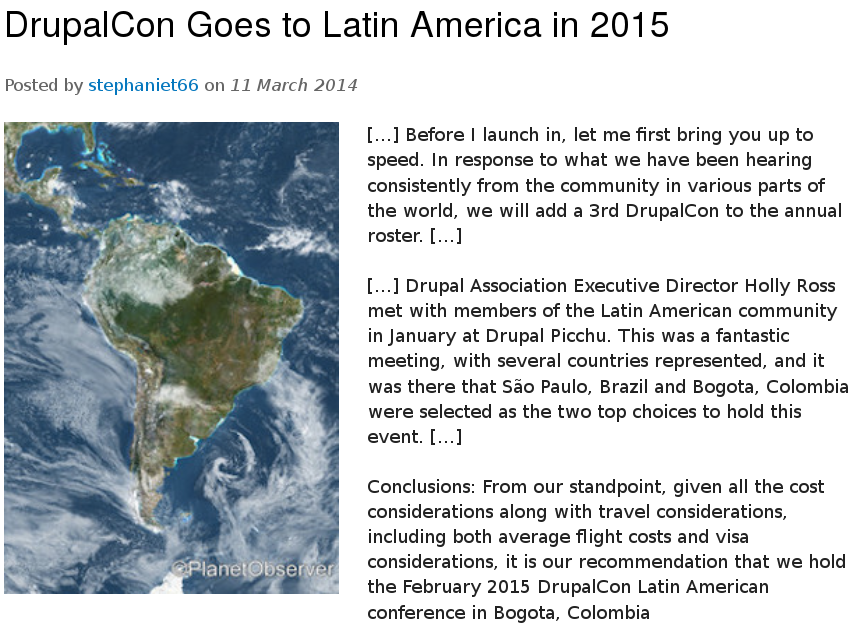
\includegraphics[width=\textwidth]{img/quotes_replacement/dcon_la_2015_01b.png}
\caption[Excerpt from the article ``\textit{DrupalCon} Goes to Latin America in 2015"]{Excerpt from the article ``\textit{DrupalCon} Goes to Latin America in 2015". Retrieved \nth{8} May 2017, from \url{https://assoc.drupal.org/content/drupalcon-goes-latin-america-2015}.}
\label{quote_da_dcon_la_announcement}
\end{figure}

The article received more than 250 comments in a few days, posing ardent discussions about how the decision about where \textit{DrupalCon} Latin America should be held was being made, and questioning the lack of transparency and participatory procedures to include the opinion of the community. The comment below (see figure \ref{quote_da_dcon_la_announcement_c1}) by \textsl{rafaelcichini}, who signed his comment using his position at the Drupal Brazilian institution as a manifestation of local legitimacy, illustrates an example of these tensions, in which this Drupalista strongly criticised the Drupal Association for taking a hierarchical approach for the decision-making, showing an \textit{official} preference for Bogotá, and not considering the feedback from local communities:

\begin{figure}[H]
  \centering
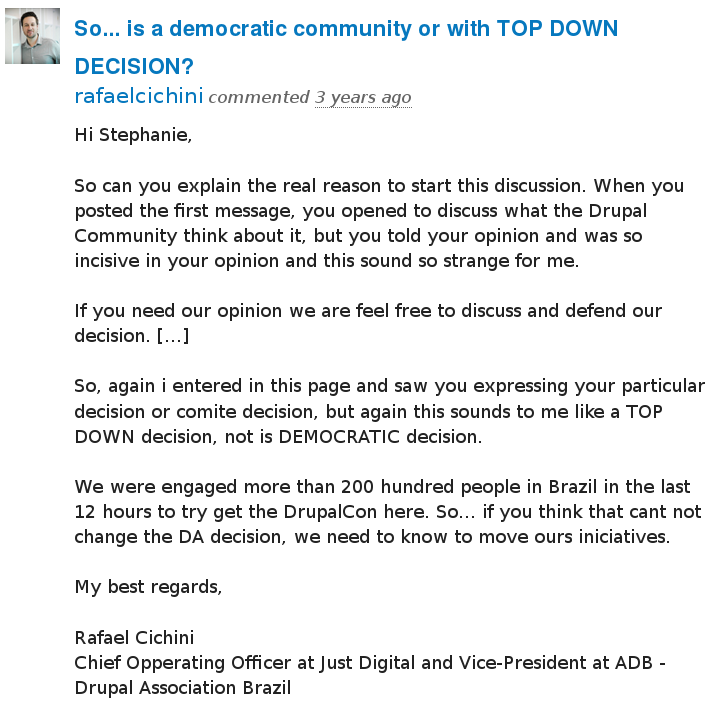
\includegraphics[scale=0.45]{img/quotes_replacement/dcon_la_2015_02.png}
\caption[Excerpt from comment (I) in the article ``\textit{DrupalCon} Goes to Latin America in 2015"]{Excerpt from comment (I) in the article ``\textit{DrupalCon} Goes to Latin America in 2015". Retrieved \nth{8} May 2017, from \url{https://assoc.drupal.org/content/drupalcon-goes-latin-america-2015}.}
\label{quote_da_dcon_la_announcement_c1}
\end{figure}

Drupalistas such as \textsl{ricardobeltranl} (see comment in figure \ref{quote_da_dcon_la_announcement_c2}) criticised the lack of possibilities for local communities to participate in this decision-making, and argued for at least clarity and transparency about how these decisions are made in a centralised way; while other Drupalistas demanded the development of more objective, clearer and more explicit criteria for these collective choices, such as depicted in the comment in figure \ref{quote_da_dcon_la_announcement_c3}, in which another Drupalista proposed the use of more quantifiable criteria for the decision.

\begin{figure}[H]
  \centering

\includegraphics[scale=0.45]{img/quotes_replacement/dcon_la_2015_03.png}
\caption[Excerpt from comment (II) in the article ``\textit{DrupalCon} Goes to Latin America in 2015"]{Excerpt from comment (II) in the article ``\textit{DrupalCon} Goes to Latin America in 2015". Retrieved \nth{8} May 2017, from \url{https://assoc.drupal.org/content/drupalcon-goes-latin-america-2015}.}
\label{quote_da_dcon_la_announcement_c2}
\end{figure}

\begin{figure}[H]
  \centering
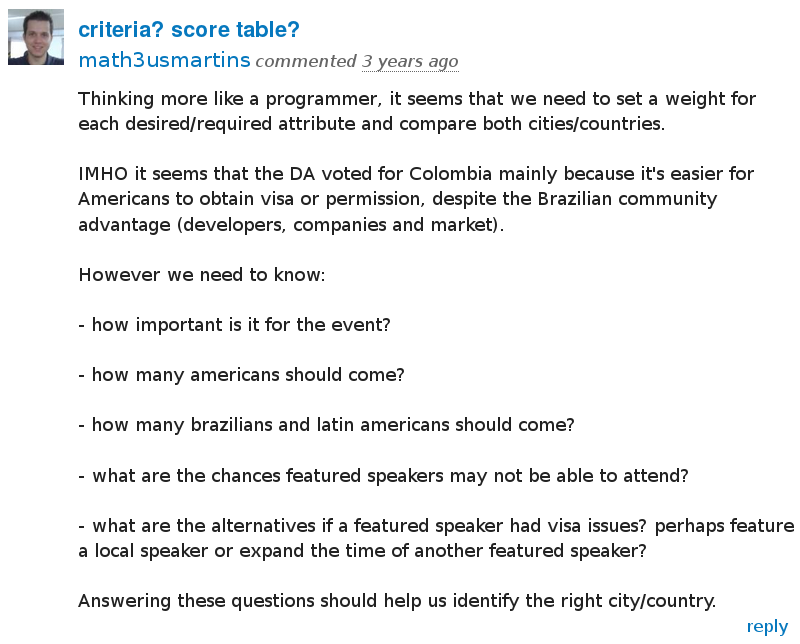
\includegraphics[scale=0.45]{img/quotes_replacement/dcon_la_2015_04.png}
\caption[Excerpt from comment (III) in the article ``\textit{DrupalCon} Goes to Latin America in 2015"]{Excerpt from comment (III) in the article ``\textit{DrupalCon} Goes to Latin America in 2015". Retrieved \nth{8} May 2017, from \url{https://assoc.drupal.org/content/drupalcon-goes-latin-america-2015}.}
\label{quote_da_dcon_la_announcement_c3}
\end{figure}

Overall, these tensions can be understood as a result of the higher degree of required legitimacy expected in this socio-technical system of contribution, in this case of the Drupal Association as an institution. These institutions are in constant pursuit of ways to improve monitoring mechanisms which increase their accountability, which are commonly achieved by means that increase the degree of formalisation. For example, an excerpt published by the Drupal Association weeks later, depicted in figure \ref{quote_da_defining_roles_02}, illustrates how these tensions operated as a source of change in the organisational processes of the Drupal Association that would be reflected, for example, in the rules and the division of labour in these organisational processes:

\begin{figure}[H]
  \centering
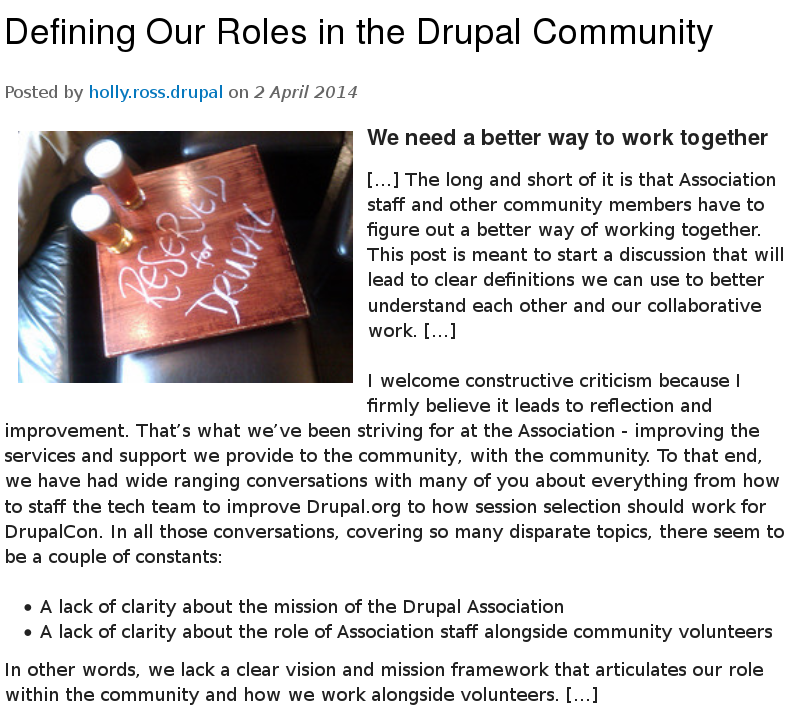
\includegraphics[width=\textwidth]{img/quotes_replacement/holly_defining_roles_2014.png}
\caption[Excerpt (II) from the article ``Defining Our Roles in the Drupal Community"]{Excerpt (II) from the article ``Defining Our Roles in the Drupal Community". Retrieved \nth{30} May 2016, from \url{https://assoc.drupal.org/content/defining-our-roles-drupal-community}.}
\label{quote_da_defining_roles_02}
\end{figure}

A clear illustration of formalisation with regard to the division of labour and rules can be found in the extensive set of roles with specific and delimited responsibilities which were defined over time. It includes a board of directors with several specific positions, an advisory board, a board member alumni and committees to improve accountability. Picture \ref{bod}, for example, depicts the board of directors and some of their positions at the time of writing (May 2016).


\begin{figure}[H]
\centering

\includegraphics[scale=0.6]{img/offline/BoD2}
\caption[Board of Directors of the Drupal Association]%
{Board of Directors of the Drupal Association. An example of the illustration of the division of labour reflected in the artefacts. Retrieved \nth{30} May 2016, from \url{https://www.drupal.org/association/board}, under a CC-BY-NC-SA license.}
\label{bod}
\end{figure}

This increment in the degree of formalisation facilitated the decentralisation of decision-making with regard to policy-making, in a similar way as in the self-organisational processes of the previously presented contribution activities.  An example of this can be found when inspecting more exhaustively how the selection of the board of directors has evolved over time. When the Drupal Association was founded by three core members, including the BDFL\footnote{See previous footnote \ref{bdfl}.}, a division of labour was defined in the form of permanent members and the board of directors, including rules to appoint or dismiss them in the statuses \parencite{drupal-vzw-statuses:2016:Online}. For instance, regarding appointment, the original rules defined that the initial permanent members were appointed by the three founders, and these permanent members then elected the first board of directors \parencite{da-history:2016:Online}, which was in charge of policy-making.

The process of appointment was partially opened later, so any Drupalista could apply to become part of the board of directors via elections. However, the right to vote was still given only to permanent members. A further step, in congruence with the increasing need of legitimacy and openness, was defined in 2012 \parencite{drupal-elections:2016:Online}, when some of these positions (e.g. director at large) were opened to votes by the whole community\footnote{The right to vote is given to all individuals who have a drupal.org account by the time the elections begin, and who have logged in at least once in the past year.}. Figure \ref{da-election16} depicts part of the main page of candidates during the last campaign.

\begin{figure}[H]
\centering
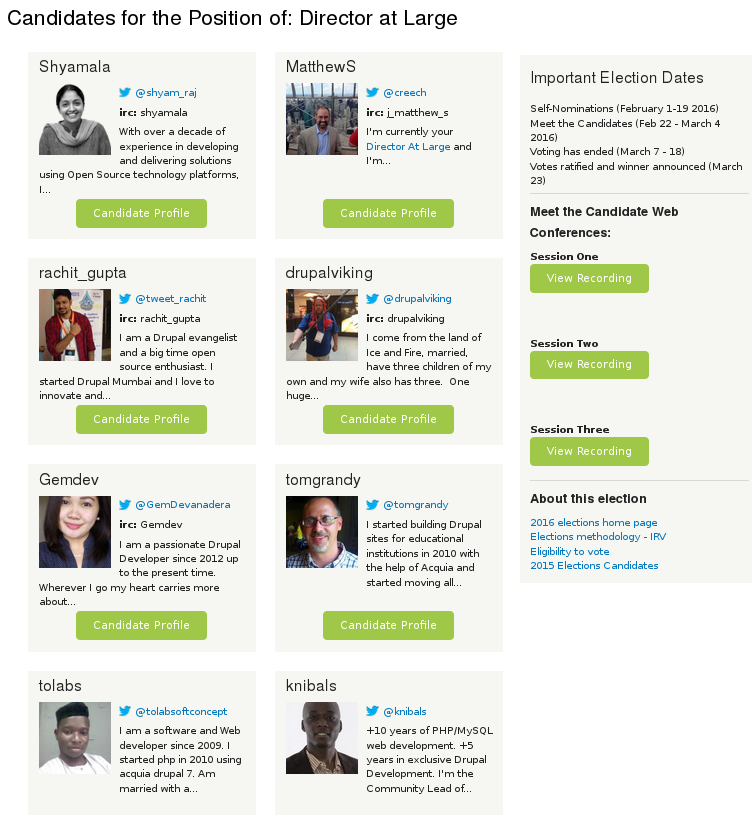
\includegraphics[scale=0.6]{img/offline/elections_16}
\caption[List of candidates to the Drupal Elections 2016 for the position of director at large]%
{Screenshot from the main page listing the candidates to the Drupal Elections 2016 for the position of director at large. Retrieved \nth{30} May 2016, from \url{https://assoc.drupal.org/election/16/candidates}.}
\label{da-election16}
\end{figure}

These changes in the organisational processes regarding decision-making are not to be misconceived as a romanticised picture of the democratisation of the Drupal Association. As it was previously stated for the case of other socio-technical systems of contribution, these dynamics are better understood as influenced by a ``do-ocratic" culture rather than a democratic one. For example, as in many other FLOSS communities, the power of the BDFL\footnote{See previous footnote \ref{bdfl}.} is still incredibly prominent in the Drupal community. However, the purpose is to illustrate how the general dynamic of formalisation found in this case study was intertwined with the increment in transparency and legitimacy of these CBPP institutions, facilitating the decentralisation of decision-making; and how this has occurred even in the most centralised, rigid and professionalised institution in the community: the Drupal Association.

This general dynamic of formalisation did not only affect the processes related to decision-making, but the organisational processes of \textit{DrupalCons} overall. For example, another illustration of the effects of formalisation on the rules that affected the organisation of \textit{DrupalCons} was the discussion and elaboration of the \textit{DrupalCon} Code of Conduct \parencite{drupalcon-coc:2016:Online}, or the creation of a Drupal Community Working Group \parencite{drupal-cwc:2016:Online} which ensures its compliance\footnote{Beyond the \textit{DrupalCon} Code of Conduct, there is a wider Drupal Code of Conduct which relates to the activities in the community overall (\url{https://www.drupal.org/dcoc}). The Drupal Community Working Group upholds them for both online and offline activities in order ``to maintain a friendly and welcoming community for the Drupal project" \parencite{drupal-cwc:2016:Online}.}. The \textit{DrupalCon} Code of Conduct summarises the shared values of the Drupal community, such as diversity, inclusiveness or self-responsibility, in order to create a safe and welcoming environment. It is usually presented during the welcoming sessions at the beginning of each \textit{DrupalCon} day, and it is also highly visible on the website and in the conference. Picture \ref{dcon-coc} illustrates a common way in which it is physically displayed at the entrance of \textit{DrupalCons}.

\begin{figure}[H]
\centering
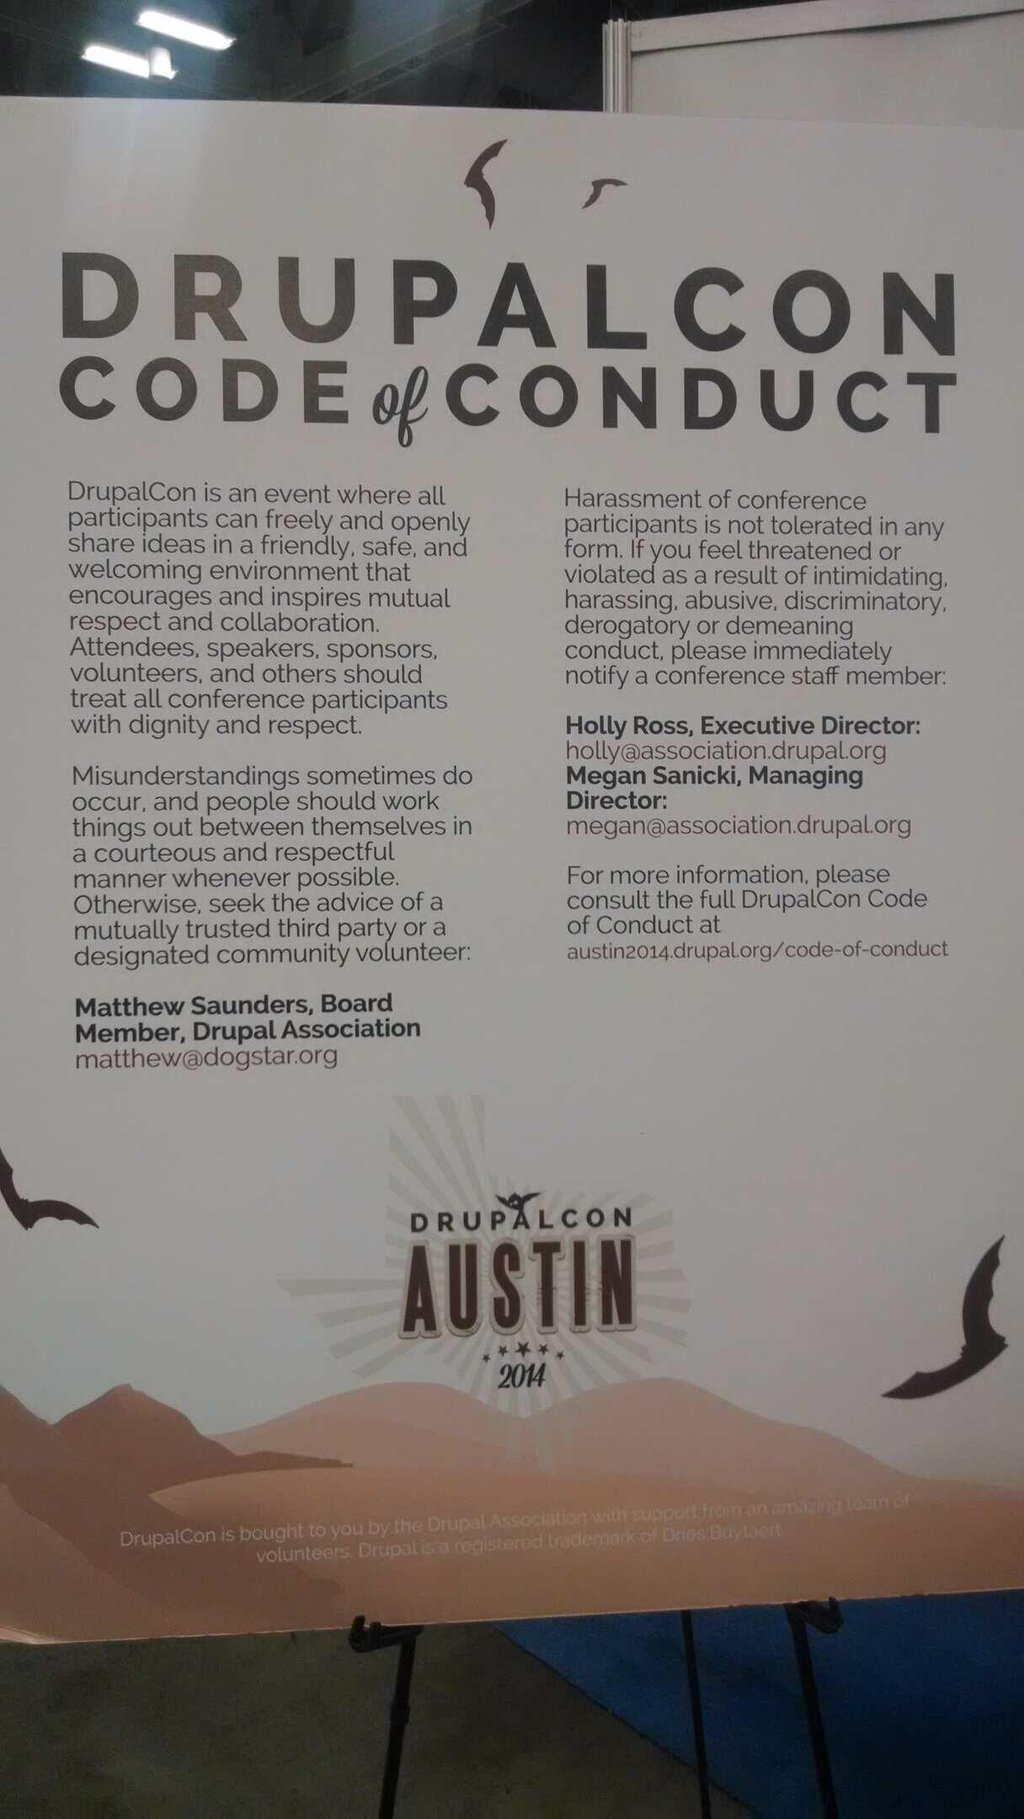
\includegraphics[scale=0.2]{img/offline/dcon_austin_coc.jpeg}
\caption[Picture from \textit{DrupalCon} Code of Conduct at \textit{DrupalCon} Austin 2014]%
{\textit{DrupalCon} Code of Conduct at \textit{DrupalCon} Austin 2014. Retrieved \nth{30} May 2016, from \url{https://twitter.com/torgospizza/status/473610332372340737}.}
\label{dcon-coc}
\end{figure}

The jurisdiction of its elaboration relied on the whole community, although it required the final approval of the Drupal Association boarding committee. The discussion took months, especially due to the difficulty to reach consensus with topics such as explicitly condemning inappropriate language, or the regulation of the consumption of alcohol on official nights due to be a possible source of a culture of exclusion. Overall, the process of elaboration of these codes of conduct represent the development of more formal conflict resolution mechanisms in accordance to rules defined by CBPP communities, and how, on occasions, they are enforced via graduated sanctions for those members who violate them. For example, the most recent application during a \textit{DrupalCon} for the time of writing occurred in New Orleans (May, 2016), when some speakers were subjected to racist, homophobic, and misogynistic comments from an anonymous Twitter account \parencite{drupal-cwc-application:2016:Online}. The incident was reported to the Drupal Community Working Group, and the person behind the account was expelled and banned from attending future \textit{DrupalCons}.

Overall, the changes experienced in the socio-technical system of \textit{DrupalCons} illustrate how the organisational processes that surround this system have also been shaped by the aforementioned dynamics of formalisation and decentralisation in decision-making, even in the case of the most centralised and rigid type of institution in the Drupal community, and despite the particularity of this trend towards paid work.

In order to show in wider detail, and from a more micro perspective, how these dynamics of formalisation and decentralisation are intertwined in the day-to-day of decision-making in the socio-technical system of \textit{DrupalCons}, the focus in the next section will be placed on the study of quality assurance processes. Concretely, the selection of presentations for \textit{DrupalCons} will be explored, since it allows the establishing of comparisons between these peer-production processes of quality assurance with respect to those discussed for the previous socio-technical systems of contribution.

\subsection{Selection of presentations in ``modern \textit{DrupalCons}"}
\label{subsec:dcons-day-to-day}

Although, from the point of view of a submitter, the process of selection of presentations in \textit{DrupalCons} may seem similar to that of \textit{DrupalCamps}, which involves submitting a proposal via a form on the official site similar to that depicted in figure \ref{dcamp-submission-form}, the internal organisational processes related to these peer-production activities for quality assurance differ significantly.

In its origin, as presented in section \ref{subsec:dcons-emergence}, the process for the selection of presentations for \textit{DrupalCons} more greatly resembled that of current local events: it was carried out informally by some of the core members of the community, and it was characterised by a lack of explicit rules and division of labour related to it. The growth experienced by \textit{DrupalCons}, in attendance, complexity and number of submissions among other factors, entailed an increase in the degree of formalisation. This period coincides with that in which \textit{DrupalCons} were still organised by local communities. As discussed in section \ref{subsec:dcons-emergence}, during this stage the stronger need for the legitimacy of quality assurance processes produced a more explicit definition of rules and division of labour, while facilitating a progressing decentralisation of the decision-making to a certain extent. The following excerpt by I\textunderscript{10} provides an overview of the process during this period in which ``\textit{DrupalCons} used to be like \textit{DrupalCamps}":

\begin{quotation}
``[...] back when there were local communities running it, the Association would appoint a... kind of like the initiative leads [comparing with this role for core projects]. The Association would appoint a local chair, and basically they picked the track chairs after that."

\begin{flushright}\footnotesize{Drupal core developer, organiser of \textit{DrupalCons} and global track chair, M, 11 years.}\end{flushright}
\end{quotation}

A key aspect illustrated in this excerpt refers to how the legitimacy of the selection of the local chair was already in the hands of the recently founded Drupal Association, even during this period in which \textit{DrupalCons} were still organised by local communities. This can be understood as part of the emergence of this new socio-technical system of ``modern \textit{DrupalCons}", while it also shows how decision-making relied on less visible hierarchies when compared to current versions of \textit{DrupalCons}. These local chairs then extended this capacity to decide to other members of the community: track chairs. This entailed a significant change with respect to the initial dynamics, in which the decision was informally made in online discussions where well-known members had a louder voice, or ``featured" presentations were directly appointed by the BDFL\footnote{See previous footnote \ref{bdfl}.} hence depicting a stronger dependency on invisible hierarchies when compared to this period in which ``\textit{DrupalCons} used to be like \textit{DrupalCamps}". During this transitional period, the degree of formalisation can be considered as intermediate. For example, clearer and more explicit rules --- as those previously depicted in figures \ref{dcon_boston01} and \ref{dcon_boston02} --- needed to be discussed and defined for the selection criteria of the presentations, resembling those for current \textit{DrupalCamps}. Nevertheless, many other rules, such as those related to the selection of the selectors themselves, were still informal, implicit and mostly dependent on invisible hierarchies.

Once \textit{DrupalCons} became their ``modern" versions, the trend towards increasing formalisation became even more prominent. Figure \ref{da-dcon-selec01} provides an overview of the main stages of the process, including for presentations selection, for a ``modern \textit{DrupalCon}", which starts nine months before the event, demonstrating this increment in the degree of formalisation that resembles more that of academic conferences.

\begin{figure}[H]
\centering
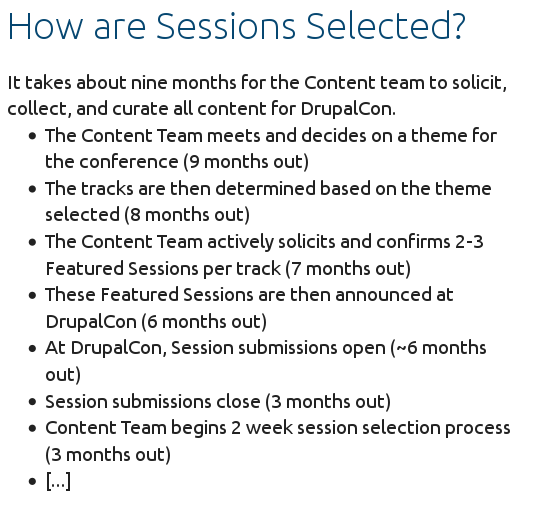
\includegraphics[scale=0.5]{img/quotes_replacement/dcon_sesssion_policy_june16_02.png}
\caption[Excerpt (I) from ``Session selection process"]{Excerpt (I) from main Drupal Association's page regarding \textit{DrupalCon}'s presentations selection policy. Retrieved \nth{20} June 2016, from \url{https://assoc.drupal.org/drupalcon/session-selection}.}
\label{da-dcon-selec01}
\end{figure}

This higher degree of formalisation responded to the same general, continuous and rising need to legitimise organisation and selection through the development of monitoring mechanisms to increase the transparency presented in section \ref{subsec:formalis-dcons}. It also facilitated the decentralisation of decision-making regarding quality assurance processes, which were needed to continuously increase the number of gatekeepers to carry out quality control, as a result of the growth in presentation submissions experienced as part of the general growth of the community --- see section \ref{sec:growth-community}. During the last few years, for example, the Drupal Association has reported the acceptance ratio for presentations to be even less than 0.05 in the most competitive tracks \parencite{drupalcon-submissions-rate:2016:Online}. Figure \ref{dcons_eu_infogram} and \ref{dcons_us_infogram} depict parts of infographics created for the Drupal Association to summarise the statistics of presentation submissions for a European (Amsterdam 2014) and a North American (New Orleans 2016) \textit{DrupalCon} respectively, providing an additional illustration of this great and increasing need for quality assurance with regards to these processes when compared to those during previous periods.

\begin{figure}[H]
\centering
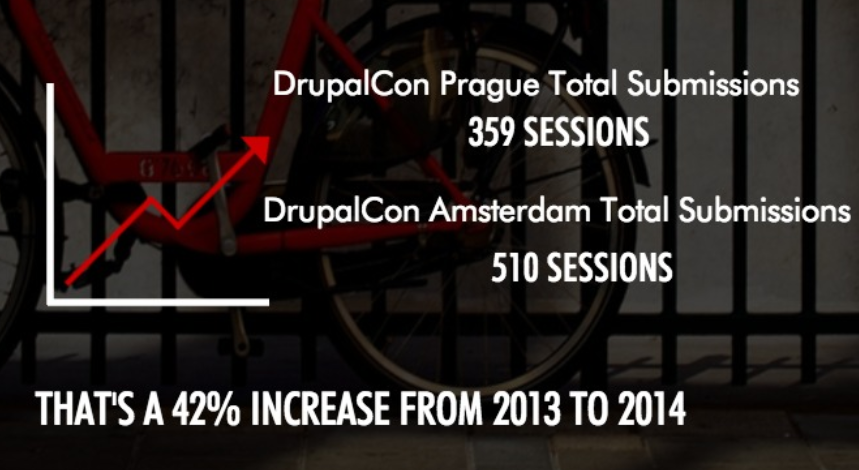
\includegraphics[scale=0.3]{img/offline/cfp_dcon_amsterdam.png}
\caption[Partial extract of an infogram about session submissions in \textit{DrupalCon} Amsterdam 2014]%
{Partial extract of an infogram about session submissions in \textit{DrupalCon} Amsterdam 2014, under a CC-BY license. Retrieved \nth{12} May 2016, from \url{https://amsterdam2014.drupal.org/news/amsterdam-session-submissions-overview.html}.}
\label{dcons_eu_infogram}
\end{figure}

\begin{figure}[H]
\centering
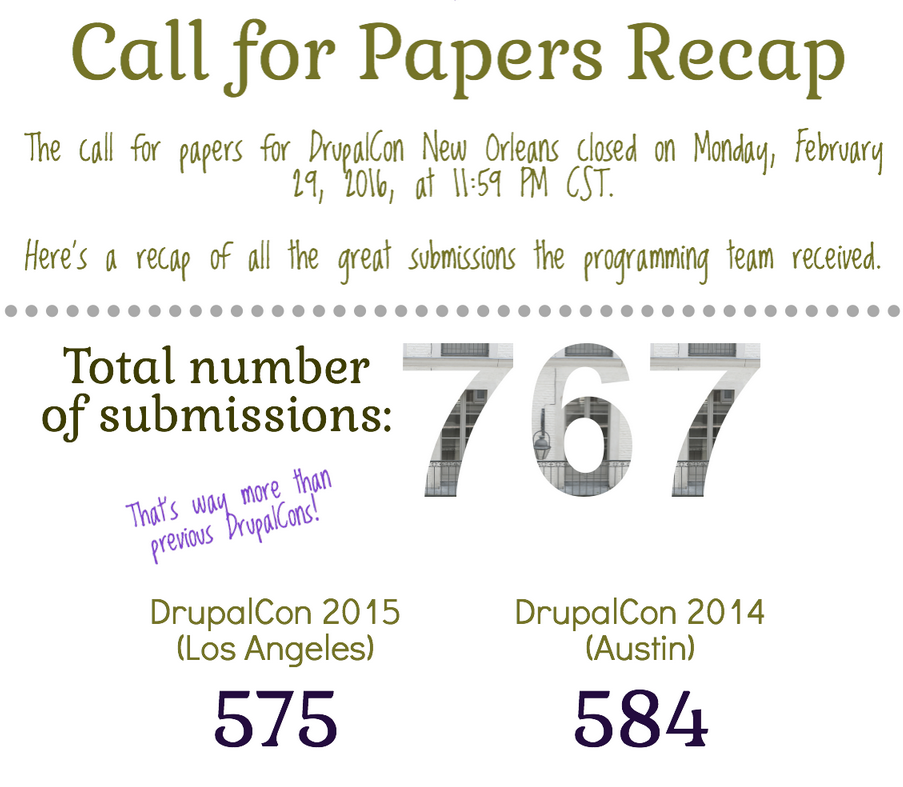
\includegraphics[scale=0.3]{img/offline/cfp_dcon_neworleans.png}
\caption[Partial extract of an infogram about session submissions in \textit{DrupalCon} New Orleans 2016]%
{Partial extract of an infogram about session submissions in \textit{DrupalCon} New Orleans 2016, under a CC-BY license. Retrieved \nth{16} August 2016, from \url{https://events.drupal.org/neworleans2016/news/record-shattering-number-session-submissions-received}. }
\label{dcons_us_infogram}
\end{figure}

The changes experienced due to growth in these self-organisational processes entailed the definition of more explicit collective-choice arrangements, increasing the degree of formalisation of the operational rules. Reflections of this can be found, for example, in the definition of explicit rules regarding the jurisdiction about who selects the submissions from the open call, or about how the decisions about ``featured" sessions  --- those skipping the general submission process --- should be made, as depicted in the extract from the \textit{DrupalCon}'s presentations selection policy in figure \ref{da-dcon-selec02}. This contrasts with how these processes were carried out in earlier stages: from being informally carried out by key members, such as the BDFL\footnote{See previous footnote \ref{bdfl}.} for the previously discussed case of \textit{merlinofchaos} in section \ref{subsec:dcons-emergence}, to rely on sets of collective-choice agreements which increase legitimacy and facilitate the distribution of the ability to make decisions to more Drupalistas.

\begin{figure}[H]
\centering
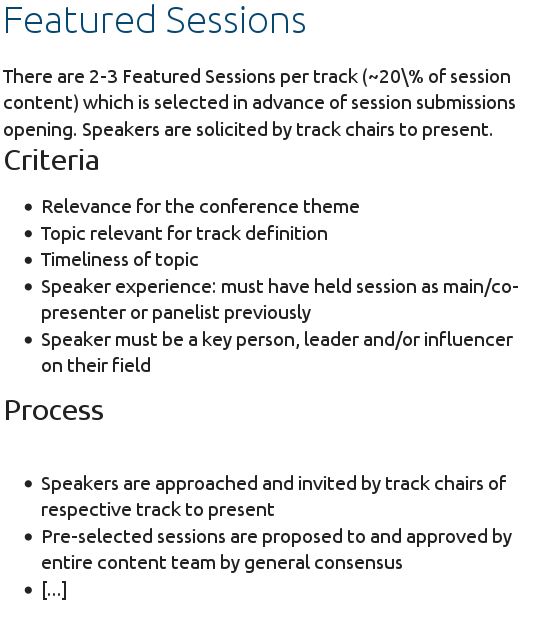
\includegraphics[scale=0.5]{img/quotes_replacement/dcon_sesssion_policy_june16_03.png}
\caption[Excerpt (II) from ``Session selection process"]{Excerpt (II) from main Drupal Association's page regarding \textit{DrupalCon}'s presentations selection policy. Retrieved \nth{20} June 2016, from \url{https://assoc.drupal.org/drupalcon/session-selection}.}
\label{da-dcon-selec02}
\end{figure}

Similarly, the dynamics of formalisation and decentralisation were also clearly reflected in the division of labour. For instance, another excerpt --- see figure \ref{da-dcon-selec03} --- from the same document for presentation selection illustrates the emergence of new and more explicit roles related to decision-making for quality assurance: a \textit{DrupalCon} content team composed of a local team (including local track chairs) and a global team (including global track chairs). This also contrasts with that of current \textit{DrupalCamps} in which, as presented in section \ref{subsec:dcamps-dtd}, there is no such division of labour, and the selection is typically carried out by all of the core organisers of the event.

\begin{figure}[H]
\centering
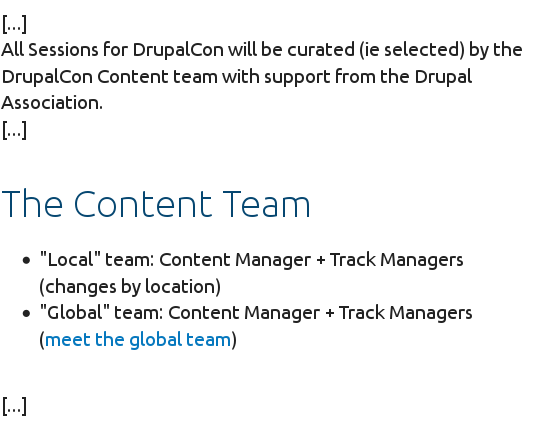
\includegraphics[scale=0.5]{img/quotes_replacement/dcon_sesssion_policy_june16_01.png}
\caption[Excerpt (III) from ``Session selection process"]{Excerpt (III) from main Drupal Association's page regarding \textit{DrupalCon}'s presentations selection policy. Retrieved \nth{20} June 2016, from \url{https://assoc.drupal.org/drupalcon/session-selection}.}
\label{da-dcon-selec03}
\end{figure}

Overall, these rules and division of labour have also become more visible for public scrutiny and discussion by the community, in contrast with \textit{DrupalCons} during previous stages. An illustration of this is the explicit reflection on the artefacts employed for collaboration (the official websites of the events), showing the aim to make these processes more visible and open for discussion. For example, the excerpt below in figure \ref{dcon-new-orleans-sp01} outlines part of the description of the selection process published on the official website of \textit{DrupalCon} New Orleans 2016:

\begin{figure}[H]
\centering
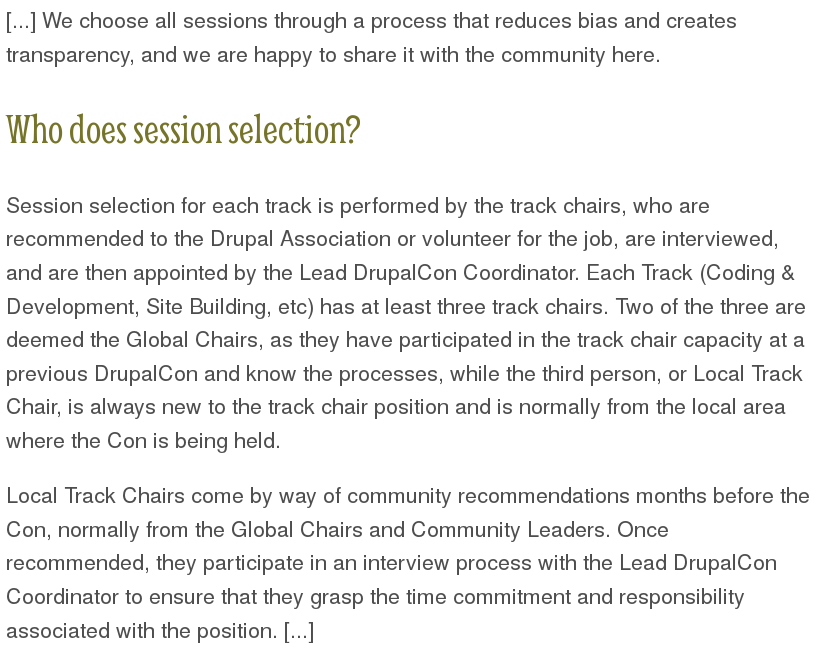
\includegraphics[scale=0.45]{img/quotes_replacement/session_selection_new_orleans_june_2016.png}
\caption[Excerpt (I) from ``Session selection process" for \textit{DrupalCon} New Orleans 2016]{Excerpt (I) from the description of the session selection process page of the main website for \textit{DrupalCon} New Orleans 2016. Retrieved \nth{21} May 2016, from \url{https://events.drupal.org/neworleans2016/session-selection-process}.}
\label{dcon-new-orleans-sp01}
\end{figure}

Another illustration of the higher degree of formalisation of this socio-technical system of contribution, which allows its comparison with those from the socio-technical systems of \textit{DrupalCamps} and local events, can be found in the rules related to regulating conflicts of interest, or in those related to tackling promotional sessions. While in local events these rules are commonly completely implicit (see section \ref{subsec:local-events}); and in \textit{DrupalCamps} intermediate levels can be observed (discussed and partially reflected in some artefacts, but not explicitly defined and regulated as presented in section \ref{subsec:dcamps-dtd}); in \textit{DrupalCons} strict policies were discussed, defined and implemented. An example of these formal and explicit rules is depicted in figure \ref{dcon-new-orleans-sp02}: an excerpt from the policy for selection of presentations published in the main artefacts for collaboration. Also, figure \ref{promotional-talks-dcons} shows the definition of specific mechanisms to deal with sessions considered promotional, in which any Drupalista can report them, as shown by the extract of a post written by a track chair reflecting on the process for \textit{DrupalCon} Amsterdam 2014.

\begin{figure}[H]
\centering
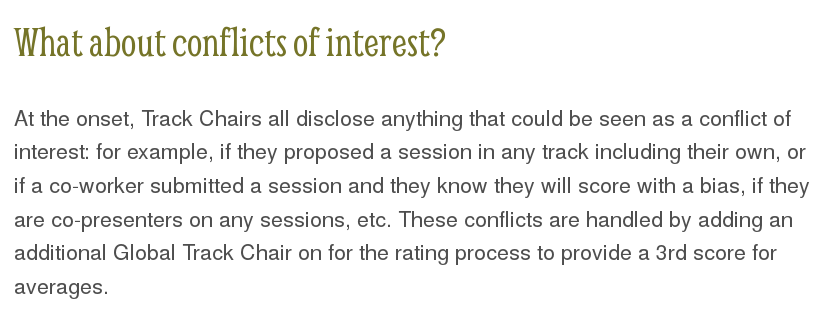
\includegraphics[width=\textwidth]{img/quotes_replacement/session_selection_conflicts_interest_new_orleans_june_2016.png}
\caption[Excerpt (II) from ``Session selection process" for \textit{DrupalCon} New Orleans 2016]{Excerpt (II) from the description of the session selection process page of the main website for \textit{DrupalCon} New Orleans 2016. Retrieved \nth{21} May 2016, from \url{https://events.drupal.org/neworleans2016/session-selection-process}.}
\label{dcon-new-orleans-sp02}
\end{figure}

\begin{figure}[H]
\centering
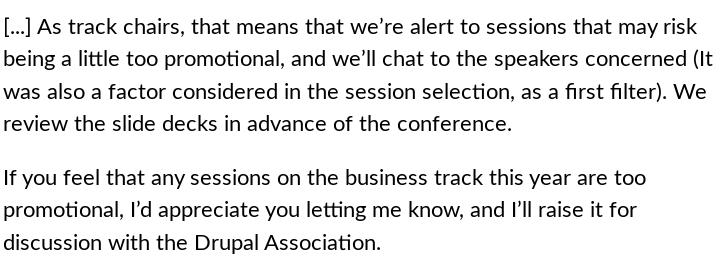
\includegraphics[scale=0.5]{img/quotes_replacement/dcon_amsterdam14_conflicts_interest.png}
\caption[Excerpt from the article ``Countdown to Amsterdam --- Shaping The Sessions After Selection"]%
{Excerpt from the article ``Countdown to Amsterdam --- Shaping The Sessions After Selection". Retrieved \nth{22} June 2015, from \url{https://amsterdam2014.drupal.org/news/countdown-amsterdam-shaping-sessions-after-selection.html}.}
\label{promotional-talks-dcons}
\end{figure}

During the interview conducted with I\textunderscript{5}, this Drupalista explained how the use of these more formal mechanisms to deal with conflicts of interest are employed in the day-to-day of these self-organisational processes, and provided an example related to the case of an employee of Acquia\footnote{Acquia is a company specialised on providing Drupal services (hosting, enterprise products or technical support among others). It was co-founded by Dries, the original creator of Drupal, and it is conceived as the largest actor in the business ecosystem around Drupal. It surpassed the 100 million dollars mark of revenue in 2014 \parencite{acquia-revenue:2016:Online}, and it was listed by Deloitte as one of the 500 fastest growing companies over two consecutive years \parencite{acquia-500:2016:Online}. The enormous growth of Acquia as a company has been a controversial topic and a source of conflict in the community, especially due to the hiring of a large number of key contributors and the impact that this could have on the general direction of the project \parencite[e.g.][]{acquia-influence01:2016:Online, acquia-influence02:2016:Online}.};

\begin{quotation}
``[...] we made use of the mechanisms for conflict of interest in the selection of presentations. For example, my global [track chair] was \textit{Daniel Johnson}, who works for Acquia. And there were many sessions from submitters working for Acquia [...]. So, we needed a third person, and he wasn't allowed to vote for any session by anyone working for Acquia. [...] As track chairs we are really strict on this. Because your reputation is at stake as well."

\begin{flushright}\footnotesize{Drupal developer, organiser of \textit{DrupalCamps} and \textit{DrupalCons}, local and global track chair, M, 9 years. Original reply in Spanish.}\end{flushright}
\end{quotation}

The organisational changes experienced in this socio-technical system of contribution not only increased the degree of legitimacy expected by the community, but they also facilitated the decentralisation of decision-making including in the most centralised and rigid of the socio-technical systems of ``mostly-offline" activities analysed. These changes entailed the creation of more autonomous spaces for decision-making, which are organised through tracks and whose rules are defined congruently with the local specificities and conditions. Rather than being defined by a central set of key members of the community as in previous stages, the evolution of these processes entailed the creation of more autonomous spaces for the decisions made by the working teams of track chairs. The following excerpt, from an interview with a Drupalista (I\textunderscript{7}) who had recently acted as local track chair for the first time, illustrates a common way in which these processes work, as well as their level of autonomy:

\begin{quotation}
``[...] we [the track chairs] voted them from 1 to 10, and we decided which kind of criteria should be taken into account. If it's a man or a woman, if she has previous experience as a speaker or not, or if she comes from a different community, for example. We decided those criteria between us [...]. And this is done for each track. Of course, we shared them... these ideas. And other tracks decided to follow some of them, others didn't. But it's not mandatory. For example, whether the speaker's gender should be taken into account or not... in order to be more gender neutral. Or whether the speaker comes from a different [FLOSS] community, to increase diversity."

\begin{flushright}\footnotesize{Drupal developer and themer, local track chair in \textit{DrupalCon}, M, 6 years. Original in Spanish}\end{flushright}
\end{quotation}

For example, with regards to the previously mentioned division of labour, it can be observed how the process evolved in a way which allowed more and new Drupalistas to take part in these decisions: the figure of local track chairs became essential to foster rotation; while that of the global chairs operated to fulfil the critical aspect of transferring knowledge. The following excerpt, extracted from field notes about a conversation with an experienced Drupalista with a long experience of organising \textit{DrupalCons}\footnote{He reported to have been in the community for more than ten years, and have been a local and global track chair. This was contrasted and verified by inspecting his Drupal.org profile afterwards.} during the observation at \textit{DrupalCon} Barcelona 2015, provides an overview of how this division of labour operates to foster rotation:

\begin{quotation}
``[...] He explained to me that the criteria about who is contacted by the Drupal Association is much more open and visible than in the old days. Some people volunteer themselves by asking the Association, while others are recommended by other key members. The recommendations given to the main DrupalCon coordinator are essential, in any case. [...] For example, he explained to me that for this DrupalCon [Barcelona 2015] he was asked for advice by the Drupal Association on the basis of his experience as a local and global track chair in previous Cons. He then decided to contact \textit{María}, who has been really active in the local community, and recommended her, and she was appointed. [...] he explained that a lot of `new blood' was entering thanks to the fact that local chairs must be new for each edition. He explained that rotation is something which has been increasing, and it is widely considered as necessary and extremely positive."

\begin{flushright}\footnotesize{Excerpt from full field notes written during participant observation in \textit{DrupalCon} Barcelona 2015 (\nth{23} September 2015).}\end{flushright}
\end{quotation}

Overall, this trend of decentralisation in decision-making via formalisation facilitated the empowering of more Drupalistas even for the most rigid and centralised of the socio-technical systems of ``mostly-offline" activities analysed. As in the case of \textit{core} projects for ``mostly-online" activities, the process is not to be thought of as one of democratisation and it is far from full egalitarianism. Furthermore, as Drupalistas who have been part of the organisation of \textit{DrupalCons} commonly acknowledged, these processes should probably be more transparent and provide better mechanisms to increase participation, although overall the trend over time has been towards them becoming more open, visible and decentralised:

\begin{quotation}
``[...] Trying to push him a bit, I told him that the criteria about how these selectors are selected did not look completely clear to me, or to other people I have talked to. He replied that having seen the organisation of DrupalCons from the inside over many years, the processes are more open for discussion than ever. [...] However, he admitted that they might still be more opaque than they should, and there is a continuous effort to try to improve this. He also emphasised the fact that more people are able to participate now than in the old days. [...] From his view, while it is still much harder to get involved in this kind of top decisions in comparison with those of events such as DrupalCamps, it's more open to participation now than in old times, when it completely depended on knowing the `big guys'."

\begin{flushright}\footnotesize{Excerpt from full field notes written during participant observation in \textit{DrupalCon} Barcelona 2015 (\nth{23} September 2015)}\end{flushright}
\end{quotation}

Overall, the changes experienced by the self-organisational processes related to quality assurance in the socio-technical system of \textit{DrupalCons} illustrate how, resembling those related to quality assurance in the socio-technical system of \textit{core} projects for ``mostly-online" activities, these processes were subjected to a general dynamic of formalisation due to the need to increase legitimacy and facilitate the decentralisation of decision-making as the community was required to scale these processes up. As a result, a set of more autonomous spaces emerged when compared with those from previous periods, in the form of specific groups for each track, in which a certain degree of rotation has been fostered by the operational rules defined over time. As in the case of the socio-technical system of \textit{core} projects for ``mostly-online" contribution activities, clearer boundaries were defined and stricter, more formal quality assurance processes were implemented within these systems in which, similarly, contributions that are part of these socio-technical systems are commonly internally perceived as more valuable than those of \textit{DrupalCamps} or \textit{contributed} projects. Even in these most rigid and centralised cases, the trend with regards to changes in decision-making has also been towards a greater degree of decentralisation over time.

\section{Conclusion}

Throughout this chapter, the emergence of and changes experienced over time in the socio-technical system of \textit{DrupalCons} were explored. This concludes the study of socio-technical systems of contribution in the Drupal community. This system represents the most rigid, valued and centralised of those studied for ``mostly-offline" activities. Nevertheless, resembling the socio-technical system of \textit{core} projects for ``mostly-online" activities, the necessity to scale up these processes also entailed a dynamic of formalisation in order to increase legitimacy, and facilitate the decentralisation of decision-making over time.

Several stages were identified with regards to the changes experienced in these general organisational processes: an initial stage in which the system operated on the most ``do-ocratic" basis, resembling current local events; a stage of transition, in which more formalised collective-choice arrangements were defined, more greatly resembling those of current \textit{DrupalCamps}; and a third stage in which there was a shift in the legitimacy to organise these events, giving legitimacy to the Drupal Association, the most formal and centralised institution in the Drupal community. Global CBPP institutions, such as the Drupal Association, are constantly searching for mechanisms which increase accountability, which are commonly achieved by means that led to an increase in the degree of formalisation. This trend towards formalisation also facilitated the decentralisation of decision-making to scale up these self-organisational processes, allowing the individuals and groups involved to gain greater authority and legitimacy.

Subsequently, it was explored how the general dynamics of formalisation and decentralisation shaped the macro level of this socio-technical system during this third stage, and how they were reflected in organisational changes in the division of labour, rules and main artefacts employed for collaboration, among others. To further understanding on how these dynamics of formalisation and decentralisation operate in this socio-technical system of contribution during this period at a more micro level, the processes of quality assurance were also explored, focussing similarly on the selection of presentations, since this allows the comparison between different degrees and ways in which the identified dynamics affected the self-organisational processes related to quality assurance of different socio-technical systems of contribution. Overall, the emergence of more autonomous spaces with a higher degree of rotation demonstrated a higher degree of decentralisation in decision-making when compared to previous stages, despite this socio-technical system being governed by the most centralised and rigid type of institution in the Drupal community.

Having concluded the exploration of socio-technical systems of contribution with different degrees of formality for ``mostly-online" and ``mostly-offline" activities throughout the previous four chapters, the overall changes experienced in the self-organisational processes of the Drupal community will be explained according to general theories of self-organising communities in the next chapter.